\chapter{Material And Methods}
Methodology is the systematic, theoretical analysis of the methods applied to a field of study. It comprises the theoretical analysis of the body of methods and principles associated with a branch of knowledge.

\section{Working Steps}
\begin{figure}[hbt]
%flowchart here	
  \begin{tikzpicture}[node distance=2cm]
  \node (step1) [process, xshift=2.5cm] {Selection of Project};
  \node (step2) [process, below of = step1] {Data Collection};
  \node (step3) [process, below of = step2] {Literature Review};
  \node (step4) [process, below of = step3, xshift=-3cm] {Calculation of bearing capacity};
  \node (step5) [process, right of= step4, xshift=5cm] {Calculation of Liquefaction Potential Index};
  \node (step6) [process, below of = step4, xshift=3.5cm] {Mapping both BC and LPI in QGIS};
  %now connect
  \draw [arrow] (step1) -- (step2);
  \draw [arrow] (step2) -- (step3);
  \draw [arrow] (step3) -| (step4);
  \draw [arrow] (step3) -| (step5);
  \draw [arrow] (step4) |- (step6);
  \draw [arrow] (step5) |- (step6);
  \end{tikzpicture}
  \caption{Project Flowchart}
\end{figure}

\subsection{Selection of Project}
As a matter of interest, we choose geotechnical field for our final year project. We discussed with our supervisor and attempted to try the Bearing Capacity Zonation and Liquefaction Potential Index Mapping. This project enables any future uses to find tentative bearing capacity and LPI of Kathmandu valley.

\subsection{Data Collection}
Data required for our project was SPT value and summary sheet for different locations as SPT was commonly used for bearing capacity calculation as well as LPI analysis of any place. Our data was provided by our supervisor as well as from Multilab. We collected about 104 boreholes from about 31 locations.

\subsection{Literature Review}
Detailed information about the project was needed, for that we studied various books as well as journals related to shallow foundation bearing capacity. As well as bearing capacity calculations from shear as well as deflection methods. For liquefaction we read various papers by Seed, Idris and research on Nepal earthquake 2015, etc.

\begin{wrapfigure}{r}{0.25\textwidth}
\centering
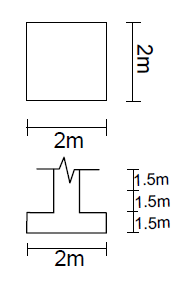
\includegraphics[width=\linewidth,keepaspectratio]{images/main/footing.png}
\caption{Footing Dimension}
\label{fsec}
\end{wrapfigure}
\subsection{Foundation Selection}
In this project work, square footing has been used. Buildings in Kathmandu valley have a depth of nearly 2m. Thus bearing capacity has been calculated for depths 1.5m, 3m and 4.5m for a footing dimension 2m * 2m as in Figure ~\ref{fsec}. Ground water table has been used as given in the bore logs. Also, the permissible settlement of 25mm is taken for settlement criteria approach.

\subsection{Calculation of bearing capacity from theoretical approaches}
The various parameters of soil like cohesion, internal angle of friction, young’s modulus of elasticity, unit weight, poisons ratio, etc were interpreted from SPT N value through various literatures available. Methods like Terzaghi, Meyerhof, Hansen, Vesic and Teng are used for the calculation of bearing capacity under shear criteria. And, Bowels, Teng, Peck and Meyerhof methods were used for settlement criteria.

\subsection{Use PLAXIS 2D for Numerical Modeling}
In this project a numerical model is developed using PLAXIS. Finite element analysis is carried out using Mohr coulomb failure criteria to represent two-dimensional soil models. Foundation is modelled as square footing and load increment is applied till the soil model fails. Ultimate bearing capacity is identified as that minimum pressure on footing at which the foundation soil experiences shear failure. And for deflection criteria, reaction at 25mm deflection is noted which is ultimate bearing capacity. In plaxis effective stress is considered as an ultimate bearing capacity.

\subsection{Calculation of liquefaction potential index}
For calculating liquefaction index, stress based approach was used and factor of safety was calculated using ratio of cyclic resistance ratio to cyclic stress ratio and from that LPI was calculated using data for up to 20m or for up to given data.

\subsection{Mapping of BC and LPI using QGIS}
We used QGIS for mapping. Map of Nepal was taken and we put our location on map. After using map of only two districts i.e. Kathmandu and Lalitpur (as our data lies on those districts). The value of all points are interpolated and clipped by our district maps. Suitable colour and map elements are selected accordingly.

IDW interpolation method was used in this software. The least value of the location was plotted. Consequently, the study area was categorized into following zones:

For Bearing Capacity:
\begin{enumerate}
\item{Weak soil region having BC $\le$ 100 kPa}
\item{Soft soil region having BC \textgreater 100 and $\le$ 150 kPa}
\item{Moderate soil region having BC \textgreater 150 and $\le$ 200 kPa}
\item{Moderately hard soil region having BC \textgreater 200 and $\le$ 250 kPa}
\item{Hard soil region having BC \textgreater 250 kPa}
\end{enumerate}

For LPI:
\begin{enumerate}
\item{Very low from 0 – 2}
\item{Low from 2 – 5}
\item{High from 5 – 15}
\item{Very high from \textgreater 15}
\end{enumerate}

\section{Determination soil properties for calculation}
\subsection{Determination of E}
The value of E can be estimated for different types of soil as given in \cite{kulhawy_manual_1990}.
\par
For cohesive soil:
\begin{equation}
\frac{E}{P_a}(kN/m^3)= \begin{cases}
    15-40 * N_{60}, & \text{for very soft soil}\\
    40-80 * N_{60}, & \text{for soft soil}\\
    80-200 * N_{60}, & \text{for compact and dense}
    \end{cases}\\
\end{equation}
\par
And for cohesionless soil:
\begin{equation}
\frac{E}{P_a}(kN/m^3)= \begin{cases}
    5 * N_{60}, & \text{with fines}\\
    10 * N_{60}, & \text{without fines}
    \end{cases}\\
\end{equation}

\subsection{Determination of C}
The values of C is determined by using Equation ~\ref{cu-form}. For cohesionless soil this value is taken as 0.

\subsection{Determination of $\phi$}
The value of $\phi$ is determined by using Equation ~\ref{phi-form}. For cohesive soil this value is taken as 0.

\subsection{Determination of $\nu$}
The value of $\nu$ is taken as:-
\begin{equation}
\nu= \begin{cases}
    0.3, & \text{for cohesionless soil}\\
    0.45, & \text{for cohesive soil}
    \end{cases}\\
\end{equation}

\subsection{Determination of other parameters}
Other parameters are calculated from Emperical Formulas in subsection ~\ref{emp-form}.

\section{Removing Outliers}
The outliers were removed by calculating $Q_1$ and $Q_3$ and calculating $IQD$. Then only values that were between $Q_1 - 1.5$ ILD and $Q_3 + 1.5$ ILD were selected for further calculation like mean and standard deviation.

\section{Selection Median}
In summary Terzaghi was excluded from shear since it has no depth corrections. Meyerhof ,Hansen, and Vesic give similar results so their average was used as a value. Finally median for summary was selected from every such values in that locations.

\section{Correlation and Regression}
Pearson’s Correlation was used for correlation. The regression was obtained by fitting 1st degree polynomial. The value of Pearson’s Correlation lies between -1 to +1. where
\begin{itemize}
\item \textbf{Positive Correlation}: both variables change in the same direction.
\item \textbf{Neutral Correlation}: No relationship in the change of the variables.
\item \textbf{Negative Correlation}: variables change in opposite directions.
\end{itemize}